%!TEX root = ../main.tex

        \chapter{PPMS测量系统} % (fold)
        \label{cha:PPMS测量系统}
            器件的测量在PPMS(Physical Proerty Measurement System)中进行,为基础的二端微波测量。在PPMS中器件被冷却到2K左右,此时金属Nb进入超导态。通过网络分析仪直接测量二维平面波导的透射信号,即可在谐振腔的谐振频率处看到透射信号被吸收形成的凹陷。我利用现有的其他类型谐振腔对测量系统进行了测试,并通过拟合可得到谐振腔的相关参数。在测量系统搭建较为完善的基础上,进一步进行2.5维LC谐振腔的测量。

            \section{测量系统概述} % (fold)
            \label{sec:测量系统概述}

            实验中使用的网络分析仪为Agilent Technologies E5071C ENA series network analyzer,输出频率范围为300kHz至20GHz,下文中将简称其为VNA。


        \begin{figure}[h]
                \centering
            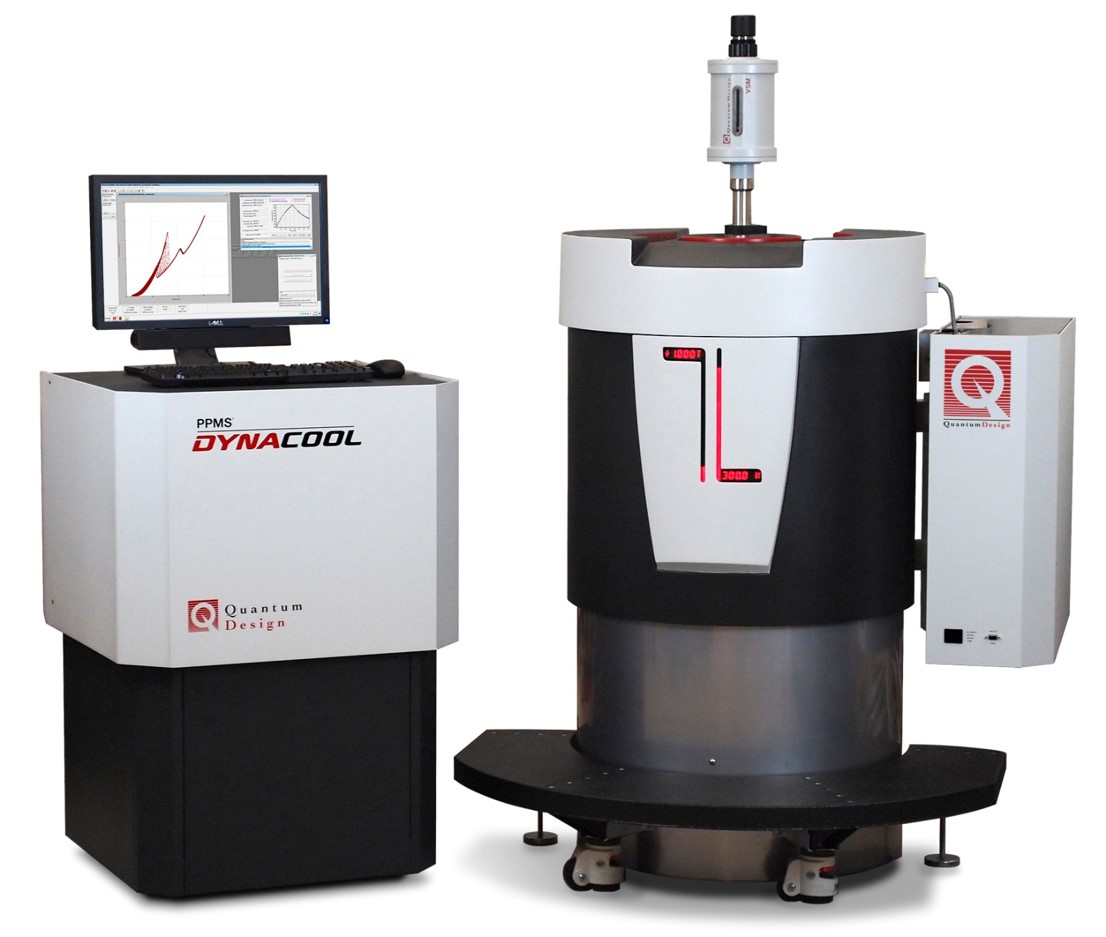
\includegraphics[width=4in]{DynaCool.jpg}
            \caption{PPMS DynaCool测量设备实物图\cite{QDDynaCool}}
            \label{fig:DynaCool}
        \end{figure}

            实验中所用的PPMS为QuantumDesign公司的DynaCool\cite{QDDynaCool},本文中都将简称它为PPMS。该PPMS可降温至1.8 K,加磁场最大为9T或14T,取决于磁体的型号。PPMS本体如图\ref{fig:DynaCool}所示,主要由控制电脑与仪器腔体两部分组成。仪器腔体的内部结构由图\ref{fig:DynaCoolStructure}所示。该图为仪器腔体在竖直平面内的横截面,可以看见样品室为被制冷环境包围住的一个立体圆柱形结构,直径不到一分米,有效的温度与磁场区域的高度大概在一分米左右。


        \begin{figure}[h]
                \centering
            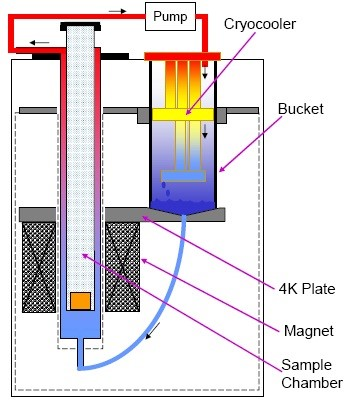
\includegraphics[width=4in]{PPMSStructure.jpg}
            \caption{PPMS DynaCool腔体内部结构\cite{QDDynaCool}}
            \label{fig:DynaCoolStructure}
        \end{figure}

            由于测量样品所在区域较小,因此无法进行需要很多端口的微波测量,但对于测量谐振腔性质所需的两个端口甚至一个端口来说较为合适。通过减小样品空间所取得的优点即在于,该PPMS系统的制冷系统长时间处于4K的低温,样品位于相对独立的样品室中,通过样品架与制冷系统的物理接触达到降温的效果,因此样品室可以较快地升温降温,而不需要对整个制冷系统进行升温降温。实际使用过程中,升温过程与降温过程所需时间均仅为30分钟左右,使得更换样品极为便捷。



            在开始本文的测量相关项目之前,该PPMS系统多用于直流测量,没有微波测量所需的设备。该部分设备的改造由交叉信息研究院孙麓岩研究组的郭星翰同学完成。改装后的样品通过样品托固定于样品杆上,进而通过样品杆插入PPMS的样品室中。由郭星翰设计的样品托如图\ref{fig:samplerodHolder}中蓝色矩形部分所示,由底座与盖子两部分组成。更换器件时,首先使PPMS样品室回到常温常压,取出样品杆,将样品托底座从盖子上拆下,再将旧样品从底座上取下,新样品安装上底座后将底座装回,插回样品杆即可。如图\ref{fig:samplerodHolder}所示,所测量的器件大小为4mm~x~7mm,放置于样品盒底座上的PCB板中央,通过点焊与PCB板相连。PCB板上焊接有两个SMP接头,与样品杆上的微波线相连并接入VNA的输入与输出端口。


\begin{figure}[h]
  \centering%
  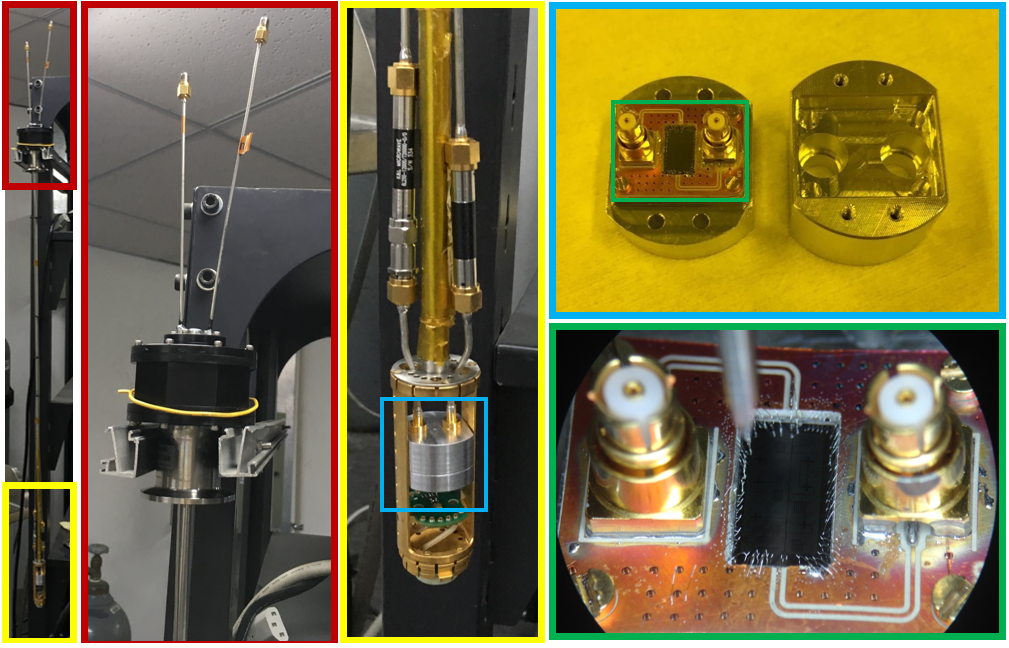
\includegraphics[width=5in]{SampleRodAndHolder.png}
  \caption{样品杆与样品盒。其中红色矩形部分为样品杆末端微波信号的输入与输出端,黄色矩形部分为样品盒所处位置,蓝色矩形为样品盒以及拆卸后的样品盒。绿色矩形内为样品盒底座上的PCB板,SMP接头以及器件及其放大图}
  \label{fig:samplerodHolder}
\end{figure}

            在实验进行过程中,我们考虑到将来进行自旋与谐振腔耦合的相关实验时需要加入竖直方向的磁场以改变自旋能级间距,而现有设计下磁场垂直与器件表面,对超导态下的器件的性质影响较大。因此,我在现有样品托的基础上改进了样品托底座与盖子以及PCB板的设计,具体在第\ref{sec:样品托的设计与优化}节中详细进行描述。
                
            % section 测量系统概述 (end)

            \section{测量系统的程序编写} % (fold)
            \label{sec:测量系统}
            通过VNA测量谐振腔的频率响应时,需要调整VNA的输出功率,IFBW,扫描频率范围,平均次数等一系列参数。这些调整步骤既可通过仪器前面板的按钮进行,也可通过远程通讯来控制。考虑到测量的便捷性,我希望通过GPIB线与VNA进行通讯并取得数据。通过Agilent提供的GPIB-USB转接头建立硬件连接,并安装Keysight Instrument Control Bundle软件后,转接头上的工作指示灯正常。Keysight Instrument Control Bundle软件提供了Keysight IO Libraries Suite软件的安装与Command Expert软件的安装。前者能够方便地查看仪器的连接状态,后者则提供仪器的SCPI指令集并可测试通过指令控制仪器。

            通过电脑与VNA建立通讯后,我以MATLAB提供的visa类为基础,通过Command Expert对VNA的相关控制指令进行了测试后,编写了通过MATLAB控制VNA的代码,具体代码可在附录\ref{cha:measurement_code}中查看。对于能够简单进行更改与询问的参数,重载了MATLAB的get与set方法。对于大范围的精细的扫描,编写了manualSweep方法,可自动将扫描范围分段进行,并返回最终扫描结果。对于数据处理环节,我将拟合相关的代码也整合进入测量阶段,进而能够节省重新导入数据的过程直接快速得到拟合结果。使用MATLAB代码进行谐振腔的测量,在1个小时内即可完成大范围搜索谐振腔的共振频率位置,对不同频率的谐振腔进行细扫并拟合得到品质因子这一系列实验步骤。以下为一部分示例代码。大部分代码采用了inputParser处理输入参数,使程序规范且易于理解。

            \begin{lstlisting}
% Example of using class E5071C
vna = E5071C('address',6);	% initialize the instrument object with GPIB address 6
vna.plotTrace;				% fetch current trace on VNA and plot in a figure
vna.freqCenter				% query and display the center frequency
vna.freqSpan = 10e6;		% set the frequency span to 10MHz
[freqs, trace] = vna.manualSweep('start',1e9,'stop',10e9,'res',1e5);	% manual sweep from 1GHz to 10GHz with 0.1MHz resolution
vna.freqCenter = 3.021e9;	% set frequency center
vna.freqSpan = 1e6;			% set frequency span
vna.plotTrace('issavedata',true,'avg',10);	% wait for 10 averages and save data while fetching the trace
vna.fit('fitall',true);		% fit the data in the current figure
            \end{lstlisting}



            对于PPMS的控制,仪器商为这台仪器提供了配套的LabVIEW程序,可以通过.NET网络协议远程控制PPMS。仪器商所提供的LabVIEW程序基于一个动态链接库文件QDInstrument.dll实现控制功能。为了通过MATLAB控制PPMS,我尝试将LabVIEW程序的VI封装成dll文件,再通过MATLAB加载与调用其中的函数。但由于LabVIEW的单个VI都会首先与PPMS建立连接,因此导致MATLAB中每调用一次PPMS的状态查看或是设置函数,就会重新建立一次连接,使程序运行缓慢,并且导致多个client同时与PPMS控制电脑上的server保持连接,可能导致潜在的问题。综合考虑后,我决定直接调用仪器商编写LabVIEW程序所调用的dll文件。

            由于不清楚QDInstrument.dll文件中程序的构成与相关接口,而这些信息是调用其中的函数所必需的。通过查询,我使用了ILSpy对该dll文件进行了反编译,结合LabVIEW程序对该dll的使用方法,确定了在MATLAB中正确调用该dll文件的方法,并以它为基础编写了通过MATLAB控制PPMS程序的代码。需要注意的是,在MATLAB中的PPMS代码的构造函数中我一添加了加载该动态链接库的MATLAB指令,但每次重启MATLAB后初始化一个PPMS实例时总是会遇到MATLAB无法找到或识别dll中应有的命名空间的错误。目前较为确定的解决办法是每次重新启动MATLAB时,需在命令行(Command Line)中手动通过NET.addAssembly方法加载dll文件,随后初始化PPMS实例。这时MATLAB仍然会报错,但此时尝试手动在命令行中输入相关内容,通过使用TAB键能够发现MATLAB已经能够识别出dll中的内容。这时再初始化PPMS实例仍然会得到报错,必须在命令行中输入调用dll中的任意对象,比如输入\mcode{QuantumDesign.QDInstrument.QDInstrumentType.DynaCool}后回车,随后再初始化PPMS实例即可成功。以下为加载dll与控制PPMS的代码示例,完整的PPMS控制代码附在\ref{sec:ppms控制代码}中。

            \begin{lstlisting}
% Example of using class PPMS
NET.addAssembly('path\to\the\file.dll');	% load the dll
ppms = PPMS;				% This will get error message. See the constructor for more parameters
QuantumDesign.QDInstrument.QDInstrumentType.DynaCool; % nothing happened, but required
ppms = PPMS;				% This time it should work
ppms.temp					% query and print the temperature
ppms.field					% query and print the magnetic field
ppms.tempStatus				% query the temperature status. It will return a QuantumDesign.QDInstrument.TemperatureStatus object
ppms.tempStatusStr			% query the temperature status. It returns a string, such as 'Chasing', 'Stable', etc.
ppms.fieldStatus
ppms.fieldStatusStr			% similar as for temperature status
ppms.setTemp(300,'tempRate',10,'tempApproach','FastSettle');		% set temperature
ppms.setField(1000,'fieldRate',100,'fieldApproach','Linear');		% set field
            \end{lstlisting}

            有了以上测量程序的编写,即可完全通过测量电脑询问与控制PPMS的温度与磁场,以及调节VNA的相关参数并取得VNA的扫描数据。更进一步的,通过Windows的远程桌面可以远程连接到测量电脑,从而使测量变得更为便捷。实际中我们只需要在取出和放入样品时到PPMS设备附近,其余时间均远程进行控制与测量。

            \section{测量系统测试} % (fold)
            \label{sec:测量系统测试}
                  对于上述PPMS测量系统,我利用自己编写的测量程序利用现有常见的CPW谐振腔进行了一系列测量测试,说明测量系统工作良好。

                  \subsection{频率扫描} % (fold)
                  \label{sub:频率扫描}
                        
                  % subsection 频率扫描 (end)

                  \subsection{温度扫描} % (fold)
                  \label{sub:温度扫描}
                        
                  % subsection 温度扫描 (end)

                  \subsection{磁场扫描} % (fold)
                  \label{sub:磁场扫描}
                        
                  % subsection 磁场扫描 (end)
            % section 测量系统测试 (end)



            \section{样品托的设计与优化} % (fold)
            \label{sec:样品托的设计与优化}



\begin{figure}[h]
  \centering%
  \begin{subfigure}{0.4\textwidth}
    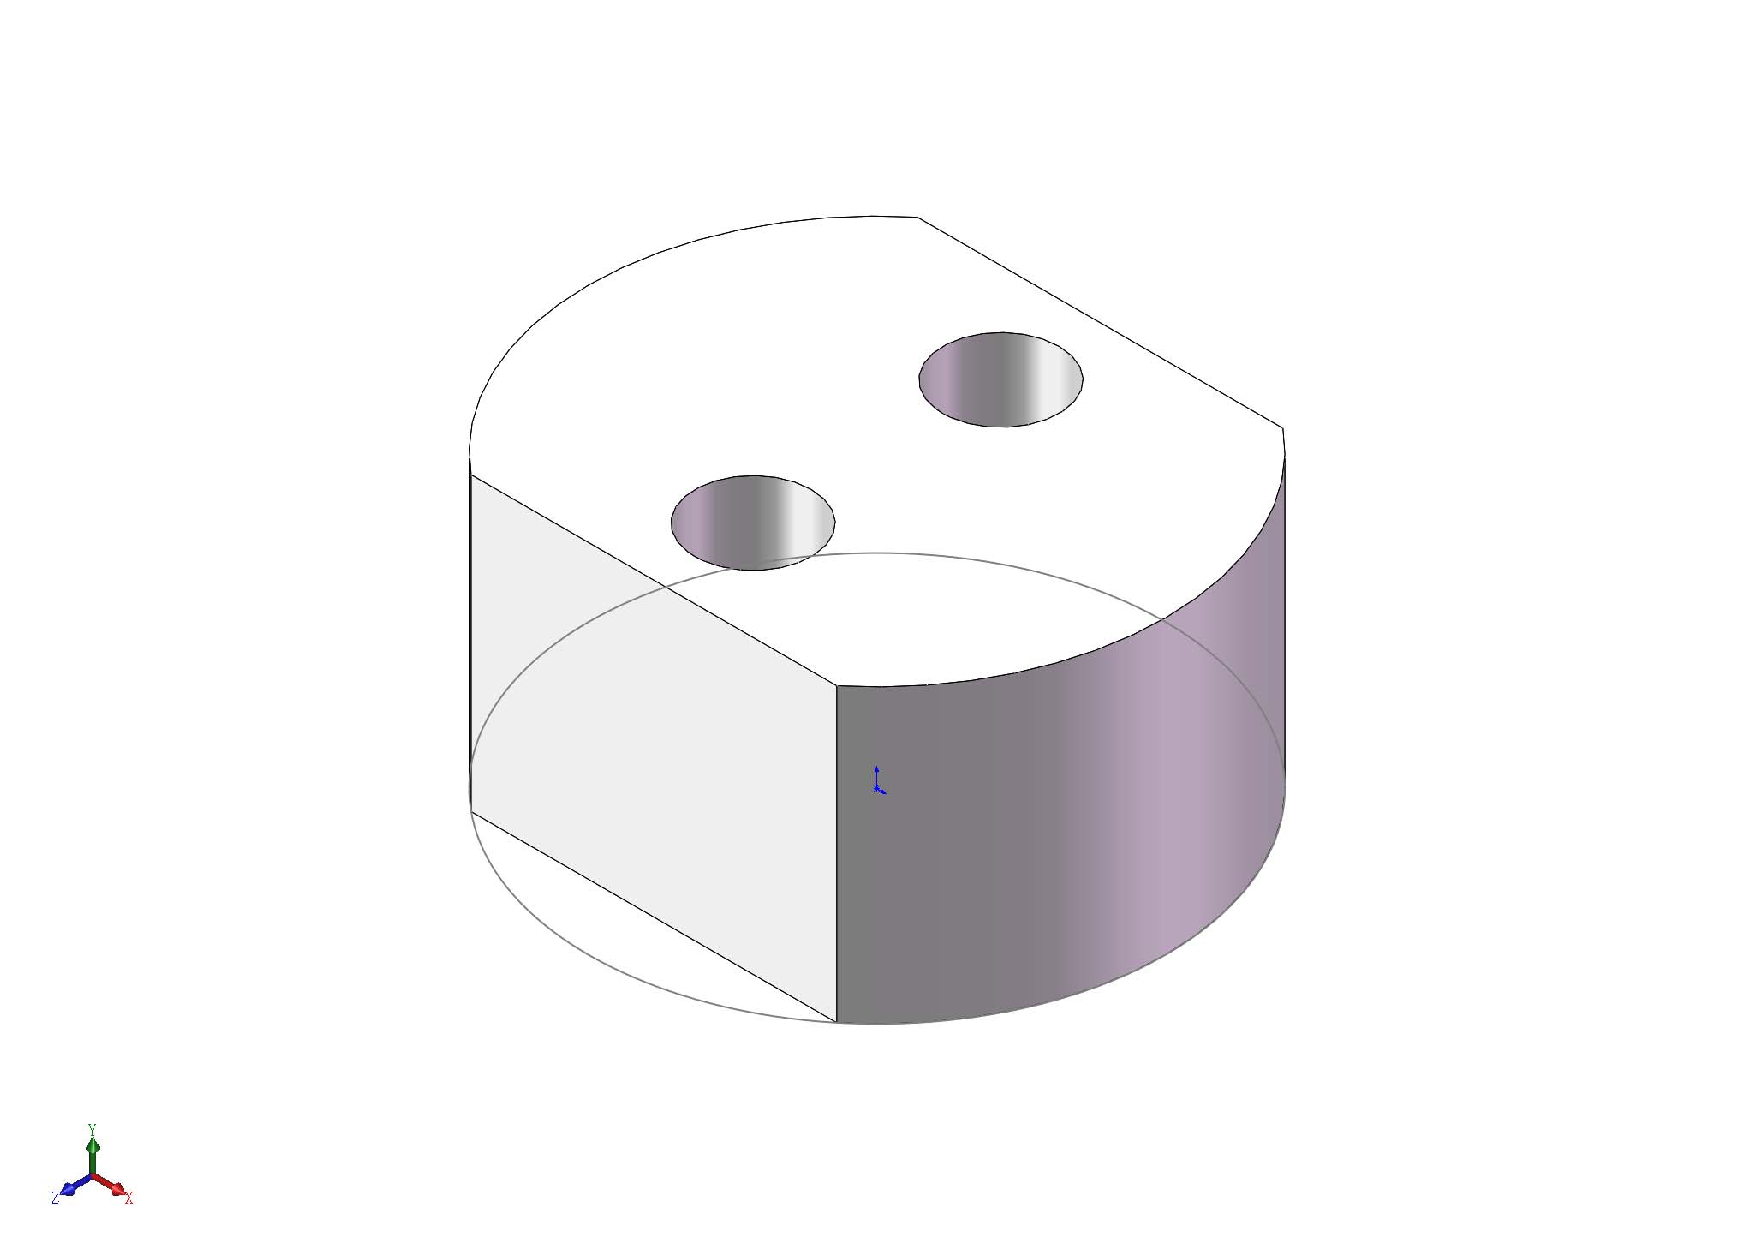
\includegraphics[width=2.2in,angle=270]{Smallbox1.pdf}
    % \caption{第一个小图形}
  \end{subfigure}%
  % \hspace{4em}%
  \hfill
  \begin{subfigure}{0.4\textwidth}
    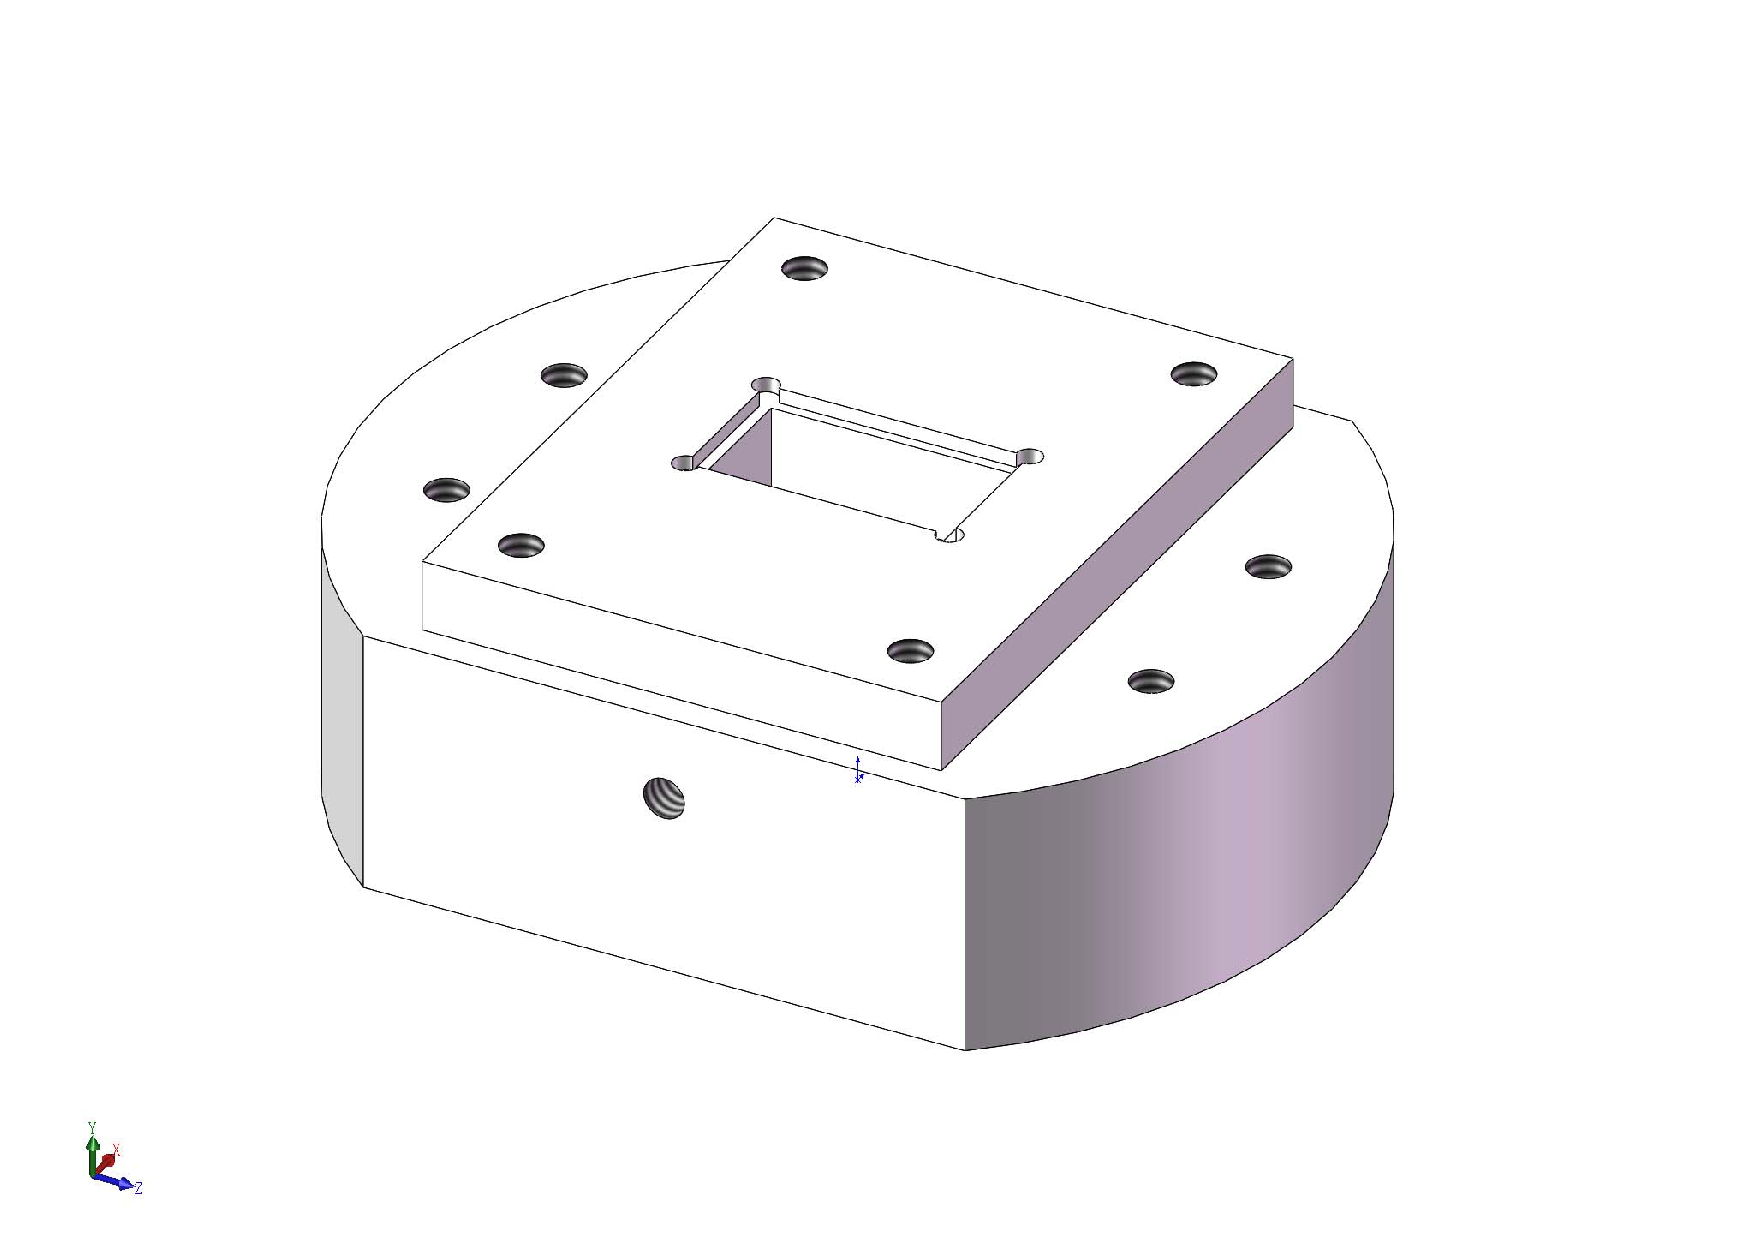
\includegraphics[width=2.2in,angle=270]{Smallbox2.pdf}
    % \caption{第二个小图形,注意这个图略矮些。subfigure中同一行的子图在顶端对齐。}
  \end{subfigure}
  \caption{原有样品盒盖子与底座设计}
  \label{fig:oldSampleBox}
\end{figure}
                  












\begin{figure}[h]
  \centering%
  \begin{subfigure}{0.4\textwidth}
    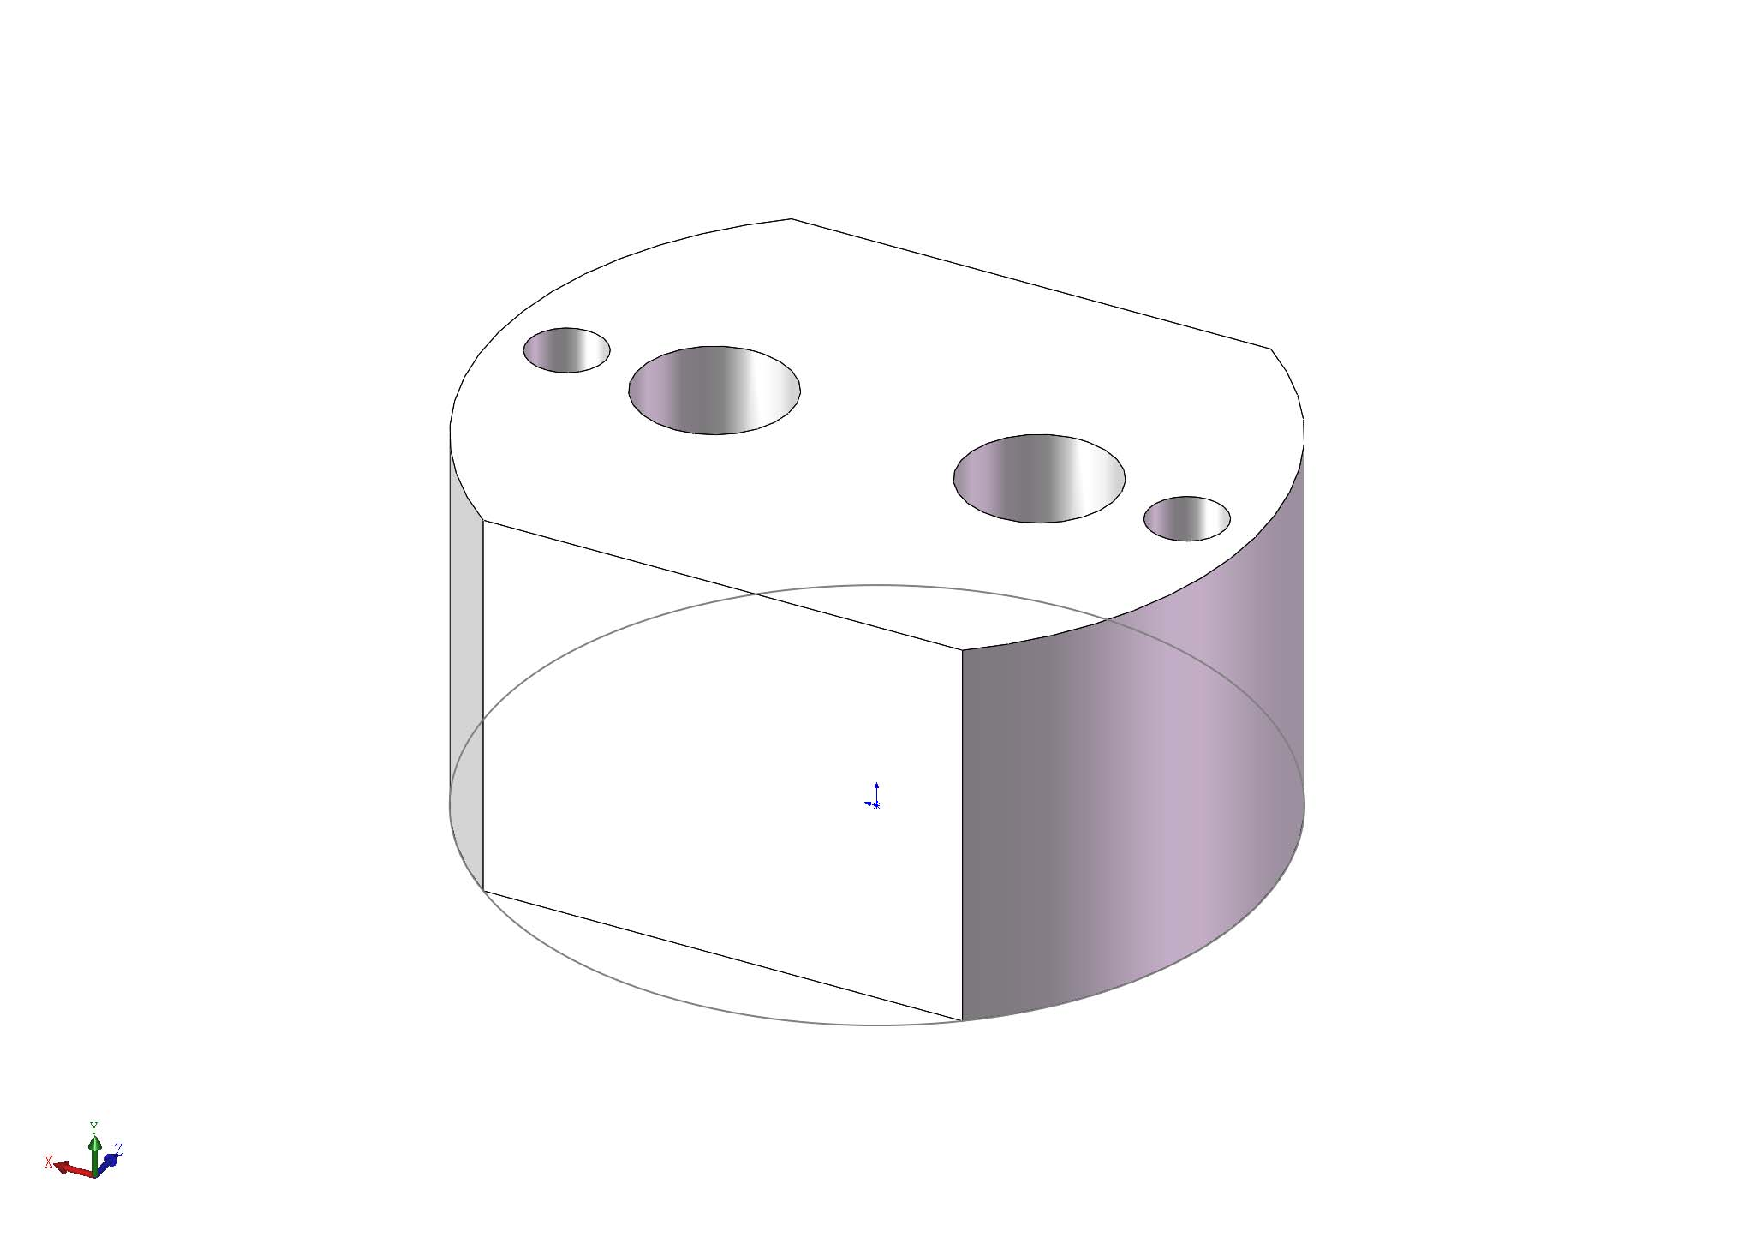
\includegraphics[width=2.2in,angle=270]{SmallboxCover.pdf}
    % \caption{第一个小图形}
  \end{subfigure}%
  % \hspace{4em}%
  \hfill
  \begin{subfigure}{0.4\textwidth}
    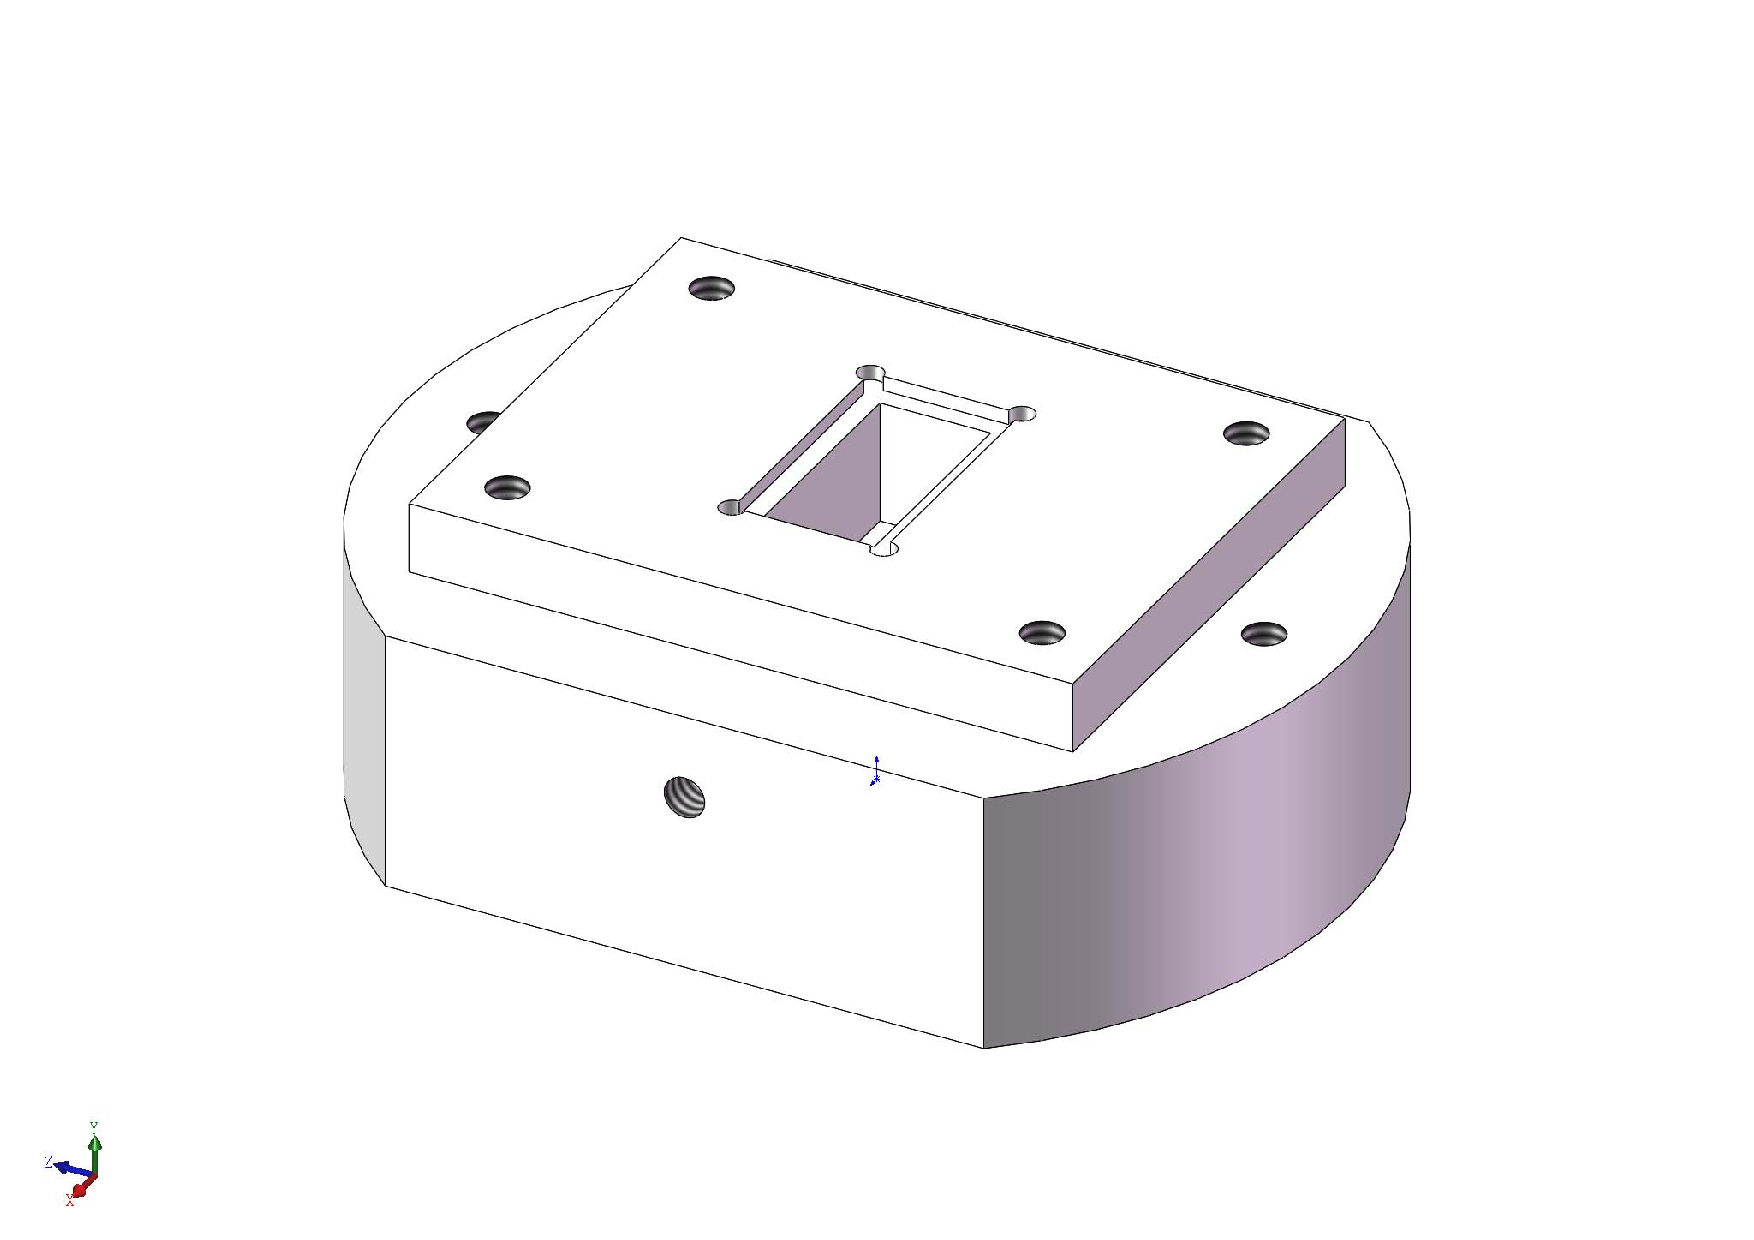
\includegraphics[width=2.2in,angle=270]{SmallboxHolderHori.pdf}
    % \caption{第二个小图形,注意这个图略矮些。subfigure中同一行的子图在顶端对齐。}
  \end{subfigure}
  \caption{改进后样品盒盖子与底座设计}
  \label{fig:newSampleBox}
\end{figure}











\begin{figure}[h]
  \centering%
  \begin{subfigure}{0.4\textwidth}
    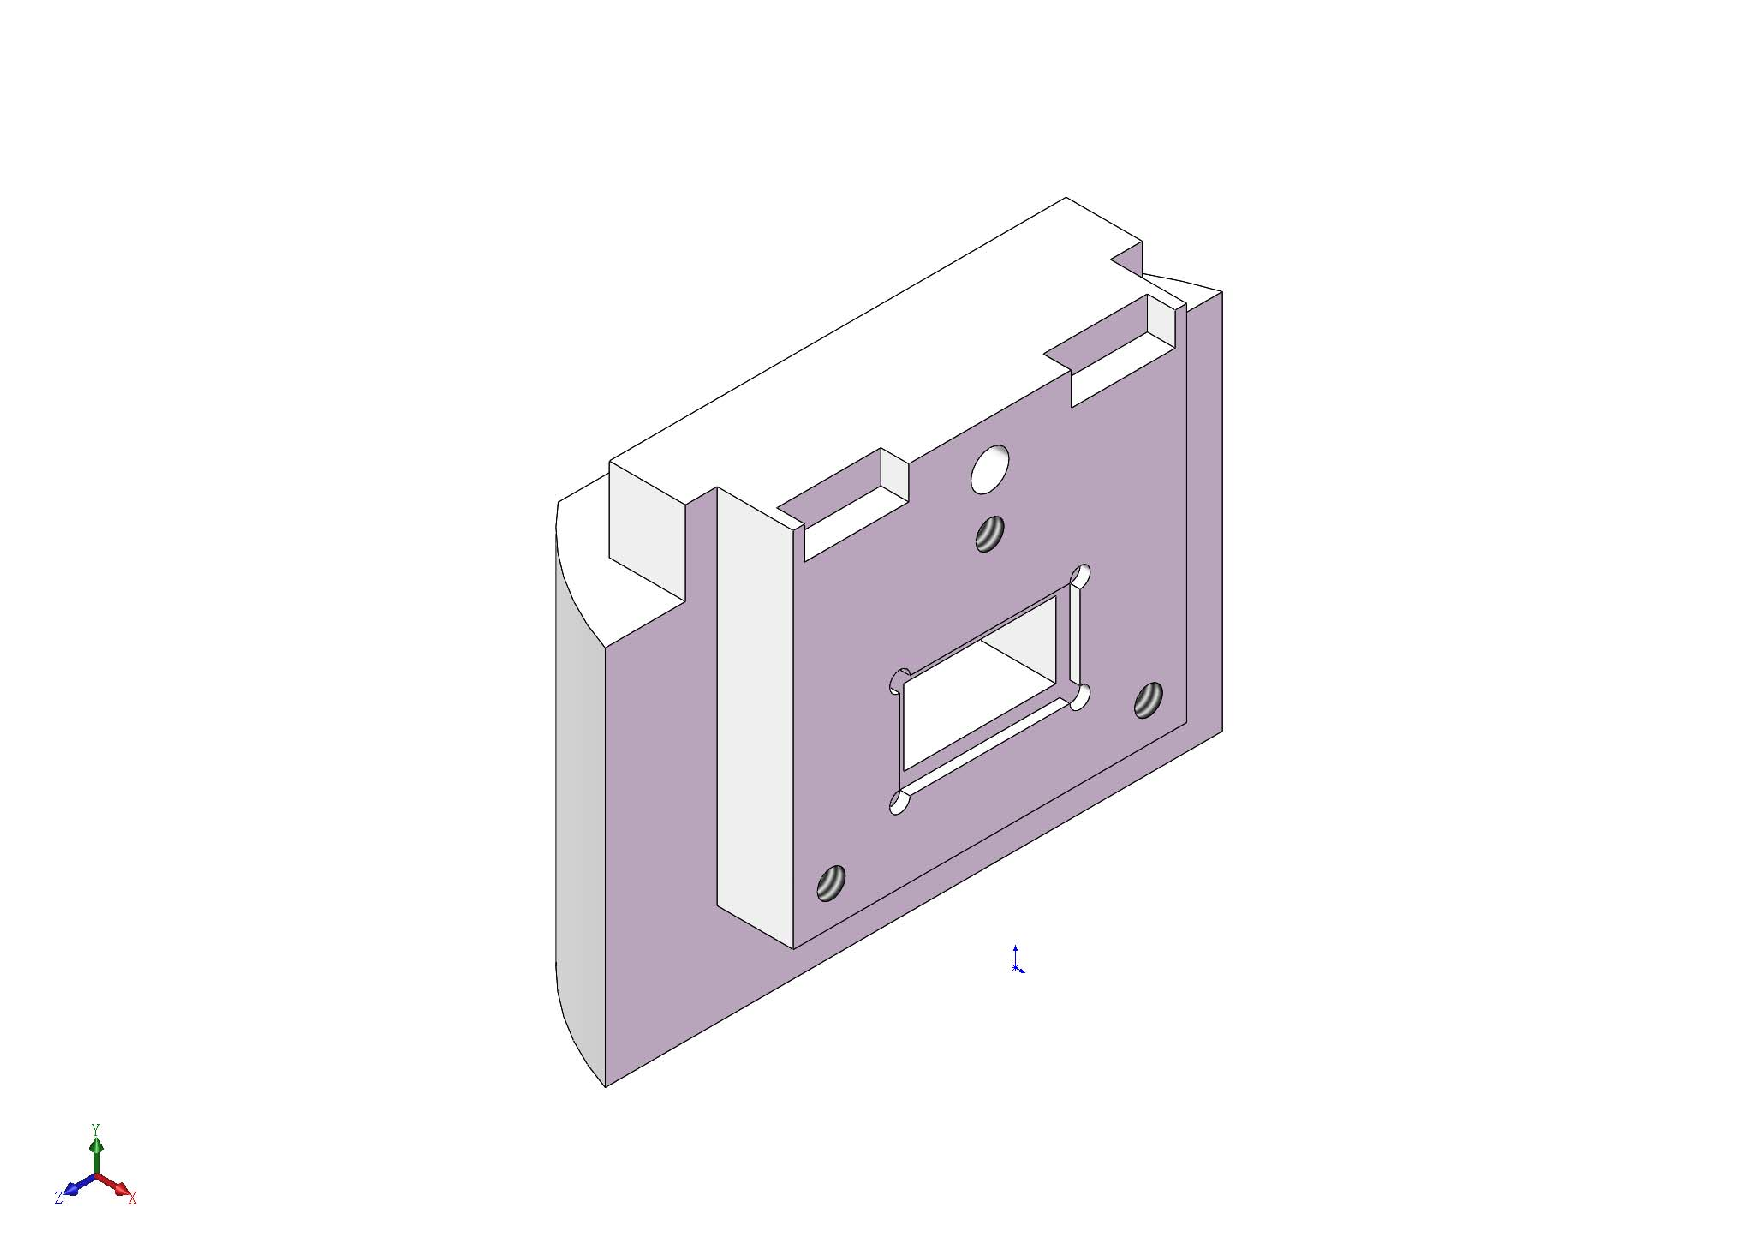
\includegraphics[width=2.2in,angle=270]{SmallboxHolderVertTotalHolder.pdf}
    % \caption{第一个小图形}
  \end{subfigure}%
  % \hspace{4em}%
  \hfill
  \begin{subfigure}{0.4\textwidth}
    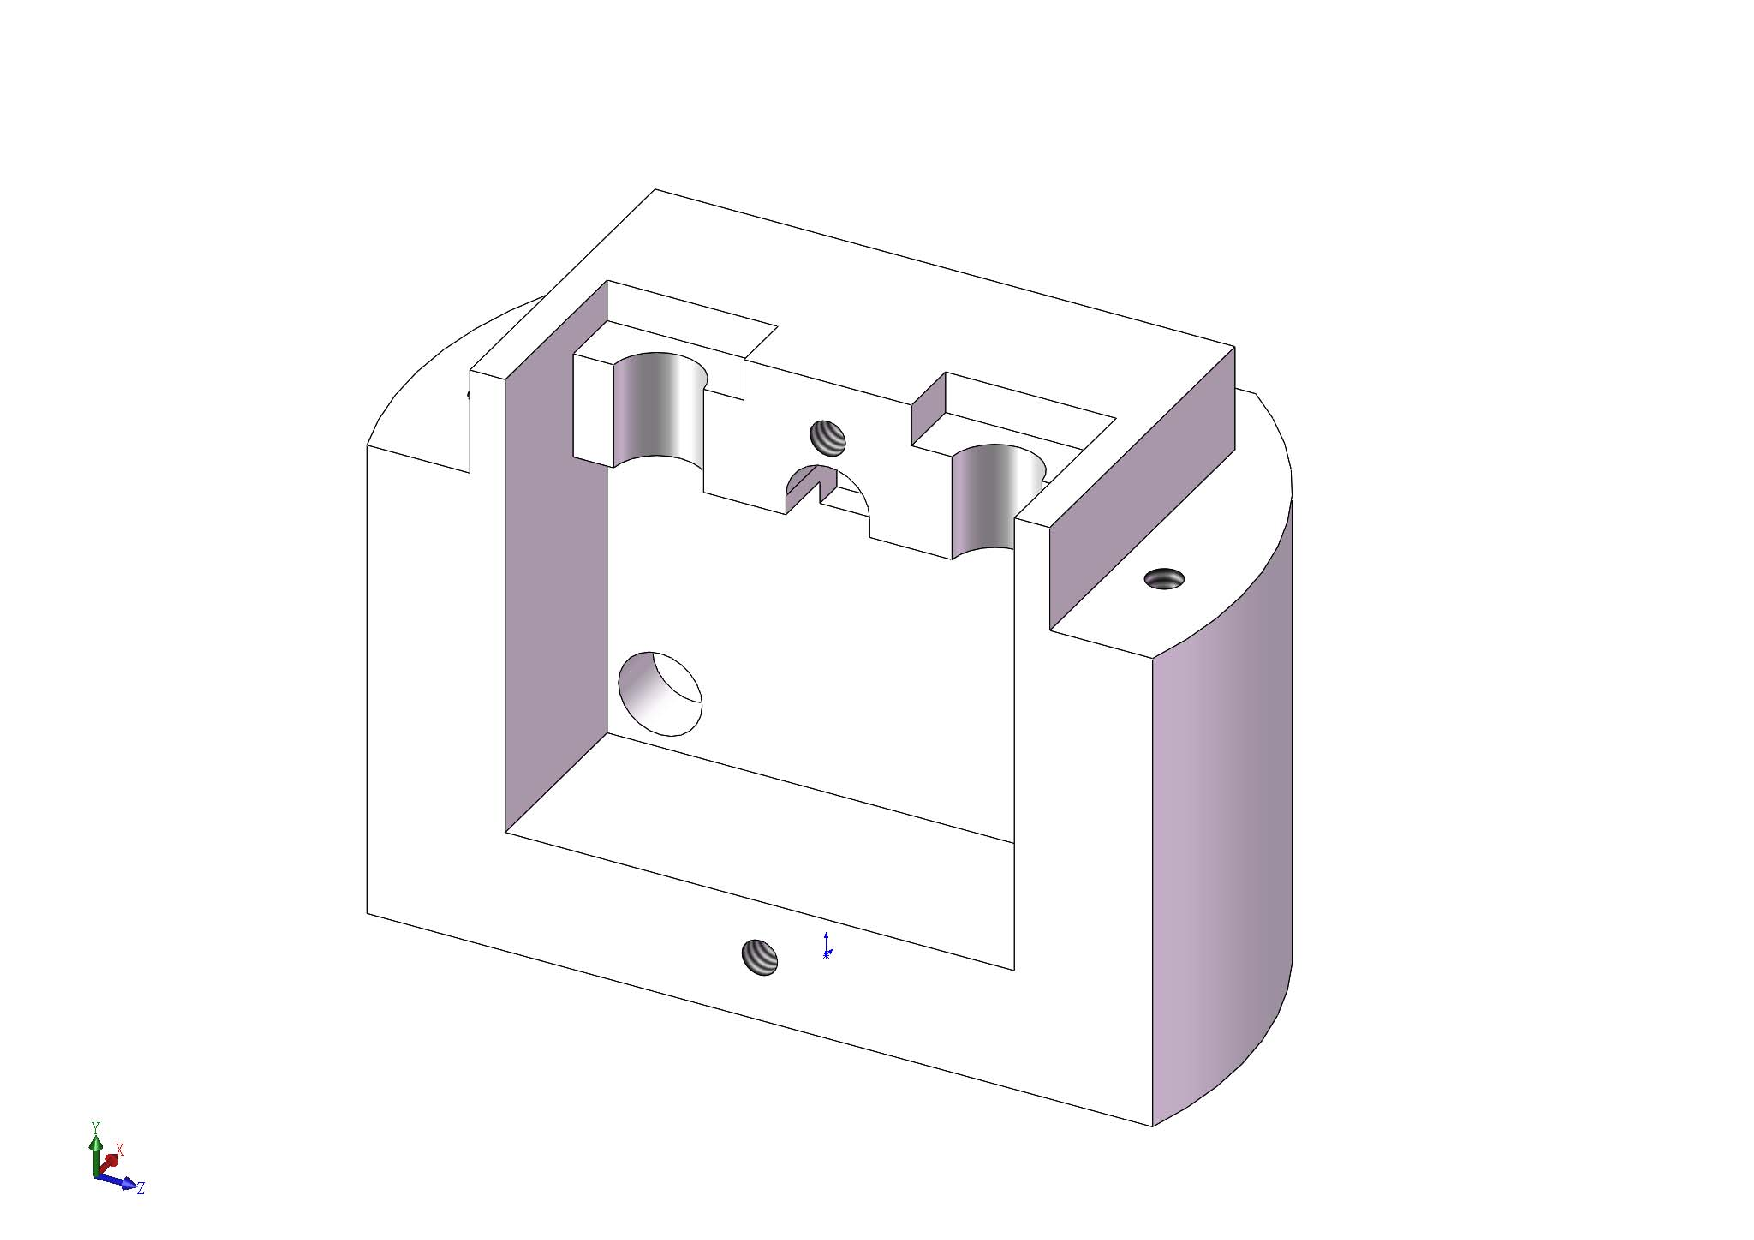
\includegraphics[width=2.2in,angle=270]{SmallboxHolderVertTotalCover.pdf}
    % \caption{第二个小图形,注意这个图略矮些。subfigure中同一行的子图在顶端对齐。}
  \end{subfigure}
  \caption{为竖直放样品所所设计的样品盒底座拆分出的盖子与底座设计}
  \label{fig:newVertiSampleBox}
\end{figure}

                  


\begin{figure}[h]
  \centering%
  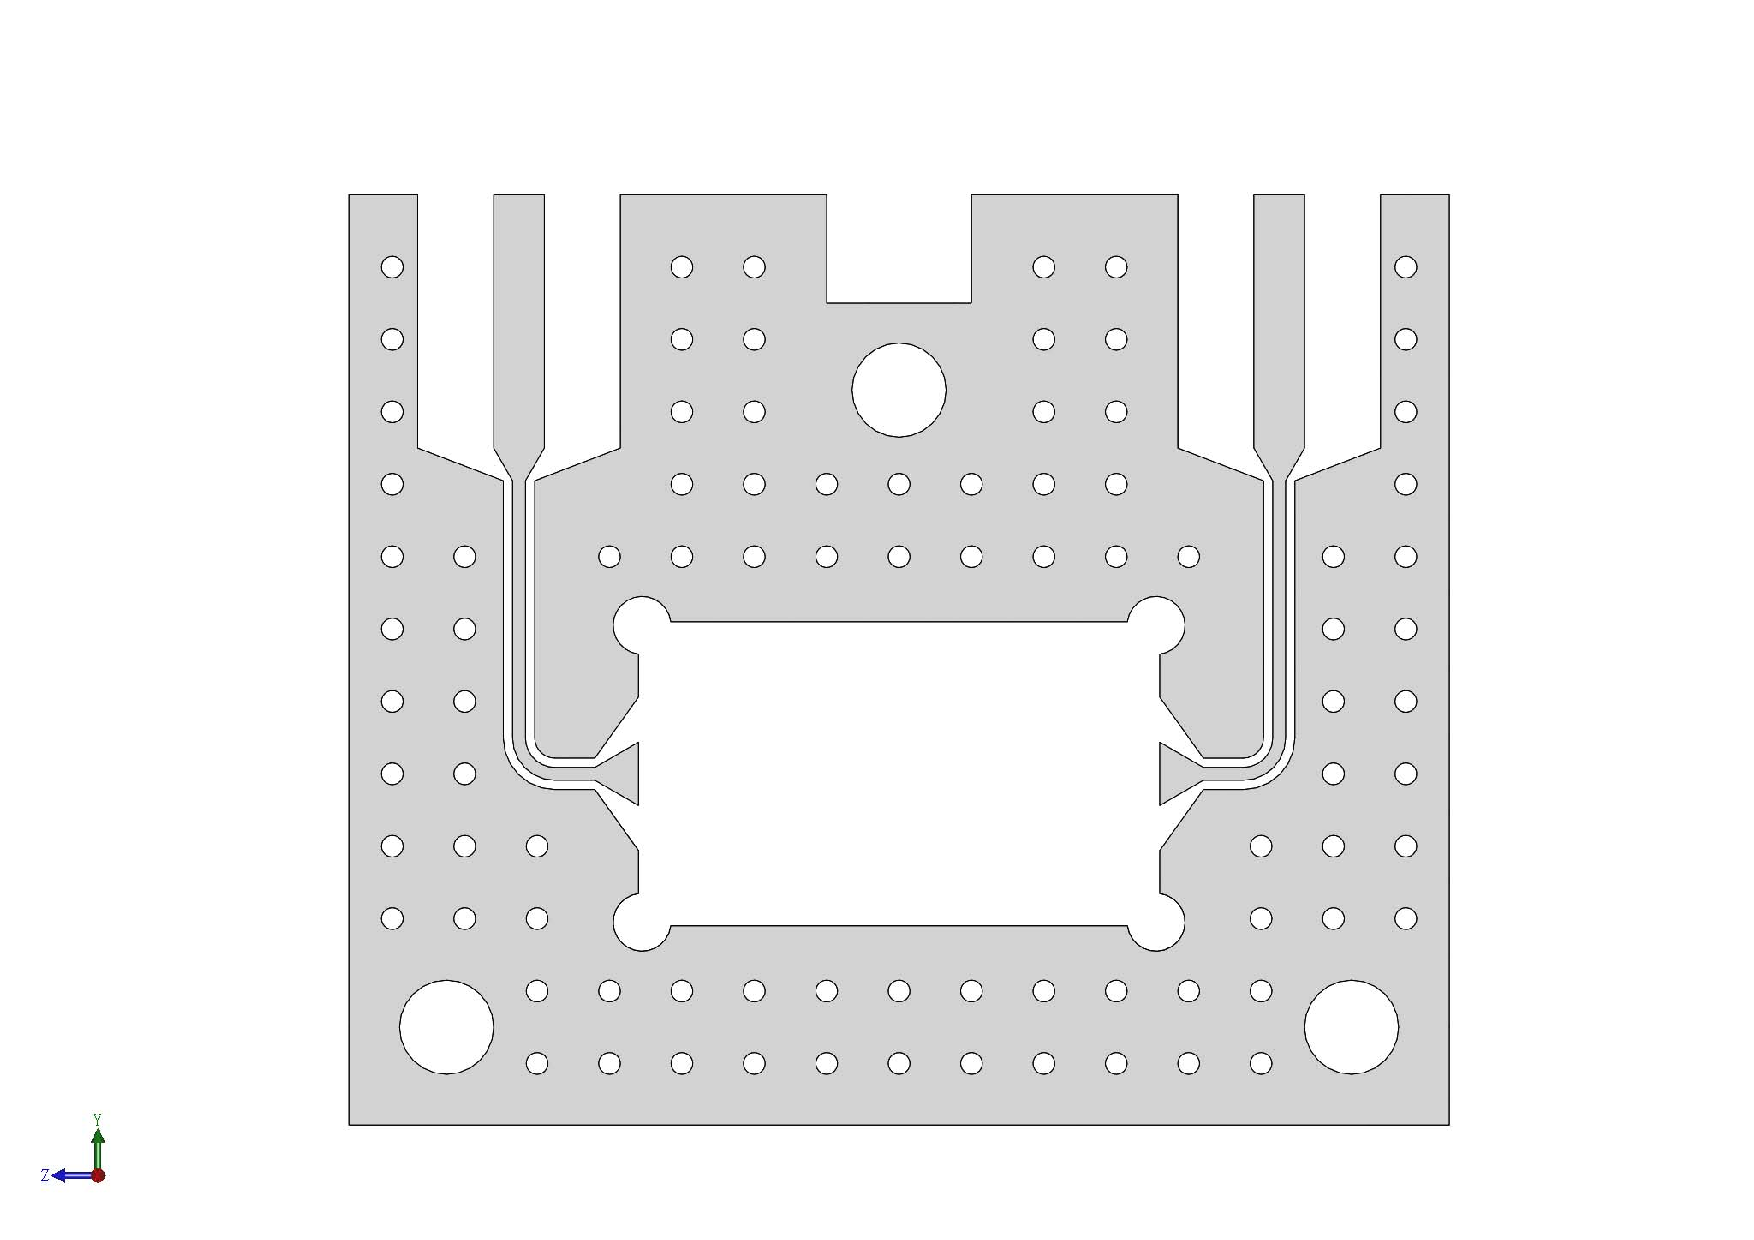
\includegraphics[width=5in,angle=270]{SmallboxHolderVertTotalHolderPCBV2.pdf}
  \caption{为新的竖直放置样品的样品盒所设计的PCB板}
  \label{fig:SmallboxHolderVertTotalHolderPCBV2}
\end{figure}






            % section 样品托的设计与优化 (end)




